\documentclass{standalone}

\usepackage{standalone}
\usepackage{tikz}
\usetikzlibrary{er,positioning}

\begin{document}
	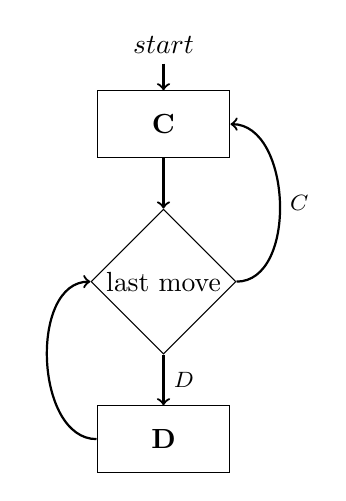
\begin{tikzpicture}[auto,node distance=1cm]

	\node[entity] (0) at (0, 0){$\textbf{C}$};
	\node (s) at (0, 1) {$start$};
	\draw (s) edge[out=-90, in=90, ->, thick] node  {} (0);

 	\node[relationship] (1) at (0, -2) {last move};
 	\draw (0) edge[out=-90, in=90, ->, thick] node {} (1);
 	\draw (1) edge[out=0, in=0, ->, thick] node [right] {\footnotesize{$C$}} (0);

 	\node[entity] (3) at (0, -4){$\textbf{D}$};
 	\draw (1) edge[out=-90, in=90, ->, thick] node [right] {\footnotesize{$D$}} (3);
  	\draw (3) edge[out=180, in=180, ->, thick] node {} (1);

	\end{tikzpicture}
\end{document}